\documentclass[aspectratio=169,11pt]{beamer}
\usetheme{Madrid}
\usecolortheme{seahorse}
\usefonttheme{structurebold}

\usepackage{listings}
\usepackage{xcolor}
\usepackage{tikz}
\usepackage{booktabs}
\usepackage{pifont}

% SQL Syntax Highlighting
\lstdefinestyle{sqlstyle}{
    language=SQL,
    basicstyle=\ttfamily\footnotesize,
    keywordstyle=\color{blue!70!black}\bfseries,
    stringstyle=\color{red!60!black},
    commentstyle=\color{green!50!black}\itshape,
    numbers=left,
    numberstyle=\tiny\color{gray},
    numbersep=5pt,
    frame=single,
    backgroundcolor=\color{gray!10},
    breaklines=true,
    showstringspaces=false,
    tabsize=2,
    morekeywords={DATABASE, REFERENCES, LIMIT, OFFSET}
}
\lstset{style=sqlstyle}

% Custom blocks
\setbeamertemplate{blocks}[rounded][shadow=true]

\title{Structured Query Language (SQL)}
\subtitle{Essential Commands \& Query Patterns}
\author{Database Systems Course}
\institute{CS Department}
\date{\today}

\begin{document}

%=============================================================================
% SLIDE 1: Title
%=============================================================================
\begin{frame}
\titlepage
\end{frame}

%=============================================================================
% SLIDE 2: Agenda
%=============================================================================
\begin{frame}{Lecture Roadmap}
\begin{columns}[T]
\begin{column}{0.5\textwidth}
\tableofcontents[sections={1-3}]
\end{column}
\pause
\begin{column}{0.5\textwidth}
\tableofcontents[sections={4-6}]
\end{column}
\end{columns}
\end{frame}

%=============================================================================
% SLIDE 3: Introduction
%=============================================================================
\section{Introduction}
\begin{frame}{What is SQL?}
\begin{block}{Definition}<1->
\textbf{Structured Query Language} is the standard language for relational database management systems (RDBMS).
\end{block}

\pause
\begin{exampleblock}{Key Categories}<2->
\begin{itemize}
    \item \textbf{DDL} -- Data Definition Language (CREATE, ALTER, DROP)
    \item \textbf{DML} -- Data Manipulation Language (SELECT, INSERT, UPDATE)
    \item \textbf{DCL} -- Data Control Language (GRANT, REVOKE)
\end{itemize}
\end{exampleblock}

\pause
\begin{alertblock}{Today's Focus}<3->
We concentrate on \textbf{querying} and \textbf{manipulating} existing data using DML commands.
\end{alertblock}
\end{frame}

%=============================================================================
% SLIDE 4: Schema Setup
%=============================================================================
\section{Basic Queries}
\begin{frame}{Sample Database Schema}
\begin{columns}
\begin{column}{0.6\textwidth}
\onslide<1->{
\textbf{Tables:}
\begin{itemize}
    \item \texttt{employees} (\underline{id}, name, dept\_id, salary, hire\_date)
    \item \texttt{departments} (\underline{id}, name, location)
    \item \texttt{projects} (\underline{id}, title, budget)
\end{itemize}
}
\pause
\textbf{Relationships:}
\begin{itemize}
    \item Employees belong to Departments (Many-to-One)
    \item Employees work on Projects (Many-to-Many via \texttt{works\_on})
\end{itemize}
\end{column}
\begin{column}{0.4\textwidth}
\onslide<3->{
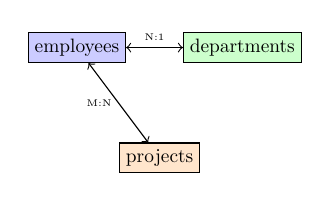
\begin{tikzpicture}[scale=0.7, transform shape]
\node[draw, fill=blue!20, rectangle] (emp) at (0,0) {employees};
\node[draw, fill=green!20, rectangle] (dept) at (3,0) {departments};
\node[draw, fill=orange!20, rectangle] (proj) at (1.5,-2) {projects};
\draw[<->] (emp) -- (dept) node[midway,above] {\tiny N:1};
\draw[<->] (emp) -- (proj) node[midway,left] {\tiny M:N};
\end{tikzpicture}
}
\end{column}
\end{columns}
\end{frame}

%=============================================================================
% SLIDE 5: SELECT Basics
%=============================================================================
\begin{frame}[fragile]{The SELECT Statement}
\begin{block}{Syntax Structure}<1->
\begin{lstlisting}
SELECT column1, column2
FROM table_name
WHERE condition;
\end{lstlisting}
\end{block}

\pause
\begin{exampleblock}{Example 1: Specific Columns}<2->
\begin{lstlisting}
SELECT name, salary
FROM employees
WHERE dept_id = 1;
\end{lstlisting}
\onslide<3->{Returns: Names and salaries for employees in department 1.}
\end{exampleblock}

\pause
\begin{exampleblock}{Example 2: Wildcards}<4->
\begin{lstlisting}
SELECT * FROM employees;
\end{lstlisting}
\onslide<5->{\textit{Caution:} Retrieves \textbf{all} columns. Inefficient for large tables!}
\end{exampleblock}
\end{frame}

%=============================================================================
% SLIDE 6: WHERE Clause
%=============================================================================
\section{Filtering Data}
\begin{frame}[fragile]{Filtering with WHERE}
\begin{columns}[T]
\begin{column}{0.5\textwidth}
\onslide<1->{
\begin{block}{Comparison Operators}
\begin{itemize}
    \item \texttt{=}, \texttt{<>} or \texttt{!=}, \texttt{<}, \texttt{>}, \texttt{<=}, \texttt{>=}
    \item \texttt{BETWEEN}, \texttt{LIKE}, \texttt{IN}
    \item \texttt{IS NULL}, \texttt{IS NOT NULL}
\end{itemize}
\end{block}
}
\end{column}
\pause
\begin{column}{0.5\textwidth}
\begin{exampleblock}{Pattern Matching}
\begin{lstlisting}
-- Names starting with 'A'
WHERE name LIKE 'A%'

-- Single character wildcard
WHERE name LIKE '_ohn'
\end{lstlisting}
\end{exampleblock}
\end{column}
\end{columns}

\pause
\begin{alertblock}{Logical Operators}<3->
\begin{lstlisting}
WHERE (salary > 50000 AND dept_id = 2)
   OR hire_date > '2023-01-01'
\end{lstlisting}
\onslide<4->{Use parentheses to control operator precedence!}
\end{alertblock}
\end{frame}

%=============================================================================
% SLIDE 7: Sorting & Limiting
%=============================================================================
\begin{frame}[fragile]{Sorting and Pagination}
\begin{exampleblock}{ORDER BY}<1->
\begin{lstlisting}
SELECT name, salary
FROM employees
WHERE salary > 40000
ORDER BY salary DESC, name ASC;
\end{lstlisting}
\onslide<2->{• \texttt{DESC}: Descending \hspace{1cm} • \texttt{ASC}: Ascending (default)}
\end{exampleblock}

\pause
\pause
\begin{block}{Limiting Results}<3->
Different SQL dialects:
\begin{lstlisting}
-- MySQL/PostgreSQL
SELECT * FROM employees LIMIT 10 OFFSET 20;

-- SQL Server
SELECT TOP 10 * FROM employees;

-- Oracle (12c+)
SELECT * FROM employees OFFSET 20 ROWS FETCH NEXT 10 ROWS ONLY;
\end{lstlisting}
\end{block}
\end{frame}

%=============================================================================
% SLIDE 8: Aggregates
%=============================================================================
\section{Aggregation}
\begin{frame}[fragile]{Aggregate Functions}
\onslide<1->{
\begin{block}{Common Functions}
\begin{center}
\begin{tabular}{ll}
\toprule
\textbf{Function} & \textbf{Description} \\
\midrule
\texttt{COUNT(*)} & Count rows \\
\texttt{SUM(column)} & Total sum \\
\texttt{AVG(column)} & Average value \\
\texttt{MAX(column)/MIN(column)} & Extreme values \\
\bottomrule
\end{tabular}
\end{center}
\end{block}
}

\pause
\begin{exampleblock}{Usage}<2->
\begin{lstlisting}
SELECT
    COUNT(*) as total_employees,
    AVG(salary) as avg_salary,
    MAX(hire_date) as newest_hire
FROM employees;
\end{lstlisting}
\onslide<3->{\textit{Note:} Aggregate functions ignore \texttt{NULL} values except \texttt{COUNT(*)}.}
\end{exampleblock}
\end{frame}

%=============================================================================
% SLIDE 9: GROUP BY
%=============================================================================
\begin{frame}[fragile]{Grouping Data}
\begin{block}{Concept}<1->
\textbf{GROUP BY} collapses rows with identical values into summary rows, typically used with aggregates.
\end{block}

\pause
\begin{exampleblock}{Department Statistics}<2->
\begin{lstlisting}
SELECT
    d.name as department,
    COUNT(e.id) as emp_count,
    AVG(e.salary) as avg_salary
FROM employees e
JOIN departments d ON e.dept_id = d.id
GROUP BY d.name;
\end{lstlisting}
\end{exampleblock}

\pause
\begin{alertblock}{The Golden Rule}<3->
Any column in \texttt{SELECT} that isn't an aggregate must appear in \texttt{GROUP BY} clause!
\end{alertblock}
\end{frame}

%=============================================================================
% SLIDE 10: HAVING Clause
%=============================================================================
\begin{frame}[fragile]{Filtering Groups with HAVING}
\begin{columns}
\begin{column}{0.5\textwidth}
\onslide<1->{
\begin{block}{WHERE vs HAVING}
\begin{itemize}
    \item \textbf{WHERE}: Filters \textit{rows} before grouping
    \item \textbf{HAVING}: Filters \textit{groups} after aggregation
\end{itemize}
\end{block}
}
\end{column}
\pause
\begin{column}{0.5\textwidth}
\begin{exampleblock}{Execution Order}
\begin{enumerate}
    \item FROM
    \item WHERE
    \item GROUP BY
    \item HAVING
    \item SELECT
    \item ORDER BY
\end{enumerate}
\end{exampleblock}
\end{column}
\end{columns}

\pause
\begin{exampleblock}{Example}<3->
\begin{lstlisting}
SELECT dept_id, AVG(salary) as avg_sal
FROM employees
WHERE hire_date > '2020-01-01'
GROUP BY dept_id
HAVING AVG(salary) > 60000;
\end{lstlisting}
\onslide<4->{Finds departments with high average salaries, considering only recent hires.}
\end{exampleblock}
\end{frame}

%=============================================================================
% SLIDE 11: JOINs Theory
%=============================================================================
\section{Joins}
\begin{frame}{Understanding JOINs}
\onslide<1->{
\begin{block}{Definition}
Combines rows from two or more tables based on a related column.
\end{block}
}

\pause
\centering
\onslide<2->{
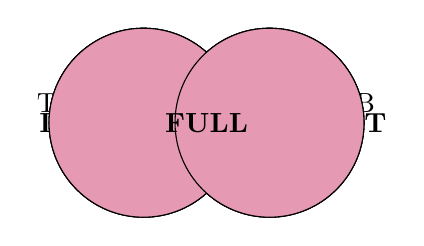
\begin{tikzpicture}[scale=0.8]
% Venn diagrams for joins
\draw[fill=blue!20] (0,0) circle (1.5cm) node[above left] {Table A};
\draw[fill=red!20] (2,0) circle (1.5cm) node[above right] {Table B};

\onslide<3->{\node at (1,0) {\textbf{INNER}};}
\onslide<4->{\draw[fill=blue!40] (0,0) circle (1.5cm); \node at (-1,0) {\textbf{LEFT}};}
\onslide<5->{\draw[fill=red!40] (2,0) circle (1.5cm); \node at (3,0) {\textbf{RIGHT}};}
\onslide<6->{\draw[fill=purple!40] (0,0) circle (1.5cm); \draw[fill=purple!40] (2,0) circle (1.5cm); \node at (1,0) {\textbf{FULL}};}
\end{tikzpicture}
}
\end{frame}

%=============================================================================
% SLIDE 12: JOIN Examples
%=============================================================================
\begin{frame}[fragile]{JOIN Syntax}
\begin{exampleblock}{INNER JOIN (Intersection)}<1->
\begin{lstlisting}
SELECT e.name, d.location
FROM employees e
INNER JOIN departments d
    ON e.dept_id = d.id;
\end{lstlisting}
\onslide<2->{Only employees with valid department IDs.}
\end{exampleblock}

\pause
\begin{exampleblock}{LEFT JOIN (Preserve Left Table)}<3->
\begin{lstlisting}
SELECT d.name, COUNT(e.id) as emp_count
FROM departments d
LEFT JOIN employees e ON d.id = e.dept_id
GROUP BY d.name;
\end{lstlisting}
\onslide<4->{Shows all departments, even those with 0 employees.}
\end{exampleblock}
\end{frame}

%=============================================================================
% SLIDE 13: Subqueries
%=============================================================================
\section{Subqueries}
\begin{frame}[fragile]{Subqueries (Nested SELECTs)}
\begin{block}{Definition}<1->
A query nested inside another query. Can appear in \texttt{SELECT}, \texttt{FROM}, or \texttt{WHERE} clauses.
\end{block}

\pause
\begin{columns}[T]
\begin{column}{0.5\textwidth}
\begin{exampleblock}{Correlated}<2->
\begin{lstlisting}
SELECT name, salary
FROM employees e1
WHERE salary > (
    SELECT AVG(salary)
    FROM employees e2
    WHERE e2.dept_id = e1.dept_id
);
\end{lstlisting}
\onslide<3->{Executes once per row.}
\end{exampleblock}
\end{column}
\pause
\begin{column}{0.5\textwidth}
\begin{exampleblock}{Non-Correlated}<4->
\begin{lstlisting}
SELECT name
FROM employees
WHERE dept_id IN (
    SELECT id
    FROM departments
    WHERE location = 'NYC'
);
\end{lstlisting}
\onslide<5->{Executes once total.}
\end{exampleblock}
\end{column}
\end{columns}
\end{frame}

%=============================================================================
% SLIDE 14: Data Modification
%=============================================================================
\section{Data Modification}
\begin{frame}[fragile]{Modifying Data}
\begin{alertblock}{\textcolor{red}{\ding{43}} Safety First}<1->
Always use \texttt{WHERE} clauses with UPDATE and DELETE, or you'll affect \textbf{all} rows!
\end{alertblock}

\pause
\begin{exampleblock}{INSERT}<2->
\begin{lstlisting}
-- Single row
INSERT INTO employees (id, name, salary)
VALUES (101, 'Alice Smith', 75000);

-- Multiple rows
INSERT INTO employees VALUES
    (102, 'Bob', 2, 60000, '2024-01-15'),
    (103, 'Carol', 2, 65000, '2024-01-20');
\end{lstlisting}
\end{exampleblock}

\pause
\begin{exampleblock}{UPDATE \& DELETE}<3->
\begin{lstlisting}
UPDATE employees
SET salary = salary * 1.05
WHERE performance_rating = 'Excellent';

DELETE FROM employees
WHERE termination_date IS NOT NULL;
\end{lstlisting}
\end{exampleblock}
\end{frame}

%=============================================================================
% SLIDE 15: Best Practices
%=============================================================================
\section{Summary}
\begin{frame}{Best Practices \& Tips}
\begin{columns}[T]
\begin{column}{0.5\textwidth}
\onslide<1->{
\begin{block}{Performance}
\begin{itemize}
    \item Use \texttt{EXPLAIN} to analyze queries
    \item Index columns in \texttt{WHERE}, \texttt{JOIN}, \texttt{ORDER BY}
    \item Avoid \texttt{SELECT *} in production
    \item Use \texttt{LIMIT} during development
\end{itemize}
\end{block}
}
\end{column}
\pause
\begin{column}{0.5\textwidth}
\begin{block}{Readability}
\begin{itemize}
    \item Use table aliases (\texttt{e}, \texttt{d})
    \item Capitalize keywords
    \item Indent subqueries
    \item Comment complex logic
\end{itemize}
\end{block}
\end{column}
\end{columns}

\pause
\begin{exampleblock}{Quick Reference}<3->
\begin{center}
\texttt{SELECT $\rightarrow$ FROM $\rightarrow$ WHERE $\rightarrow$ GROUP BY $\rightarrow$ HAVING $\rightarrow$ ORDER BY $\rightarrow$ LIMIT}
\end{center}
\end{exampleblock}
\end{frame}

%=============================================================================
% SLIDE 16: Questions
%=============================================================================
\begin{frame}
\centering
\Huge Questions? \\
\bigskip
\large Try These:
\normalsize
\begin{itemize}
    \item Find employees earning above their department average
    \item List departments with no employees
    \item Update salaries based on tenure
\end{itemize}
\end{frame}

\end{document}